\documentclass[tikz,border=10pt]{standalone}
\usepackage{amsmath}
\begin{document}
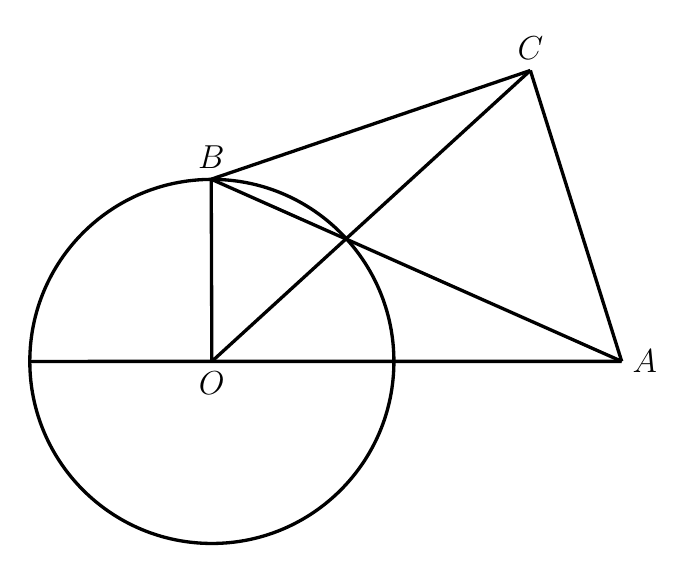
\begin{tikzpicture}[line width=1.2pt, line join=round]
  % named points (scale s = 0.014706 units/px, origin at bbox-centre-ish)
  \coordinate (O) at (-1.635,-0.838);
  \coordinate (B) at (-1.643,1.476);
  \coordinate (A) at (3.570,-0.837);
  \coordinate (C) at (2.410,2.857);
  \coordinate (D) at (0.066,0.721);
  \coordinate (L) at (-3.953,-0.838);  % left circle/line intersection

  % circle centred at O, radius 157.2 px
  \draw (O) circle[radius=2.312];

  % horizontal line through O and A (from left circle point)
  \draw (L) -- (A);

  % triangle and construction segments
  \draw (O) -- (B);
  \draw (O) -- (C);
  \draw (B) -- (C);
  \draw (C) -- (A);
  \draw (B) -- (A);

  % labels
  \node[right] at (A) {\fontsize{12.5}{15}\selectfont $A$};
  \node[above] at (B) {\fontsize{12.5}{15}\selectfont $B$};
  \node[above] at (C) {\fontsize{12.5}{15}\selectfont $C$};
  \node[below] at (O) {\fontsize{12.5}{15}\selectfont $O$};
\end{tikzpicture}
\end{document}